\section{Results}

\subsection{}

This should contain some quantitative evaluation of the robot performance. For example: that it can find a resource site from a disance of x metres, and recognise and leave within t seconds; etc.

If your robot is not capable of doing the final task, you should evaluate what it does do correctly, and try to analyse what it does wrong.

The reader should be left with an accurate understanding of exactly what your robot is capable of, even if this is not as good as you hoped. Bad results are results too. You get marked based on how you approached the problem and how you evaluated the results. (800 words)

% - - - - - - - - - - - - - - - - - - - - - - - - - - -

\begin{figure}[ht]
    \centering
    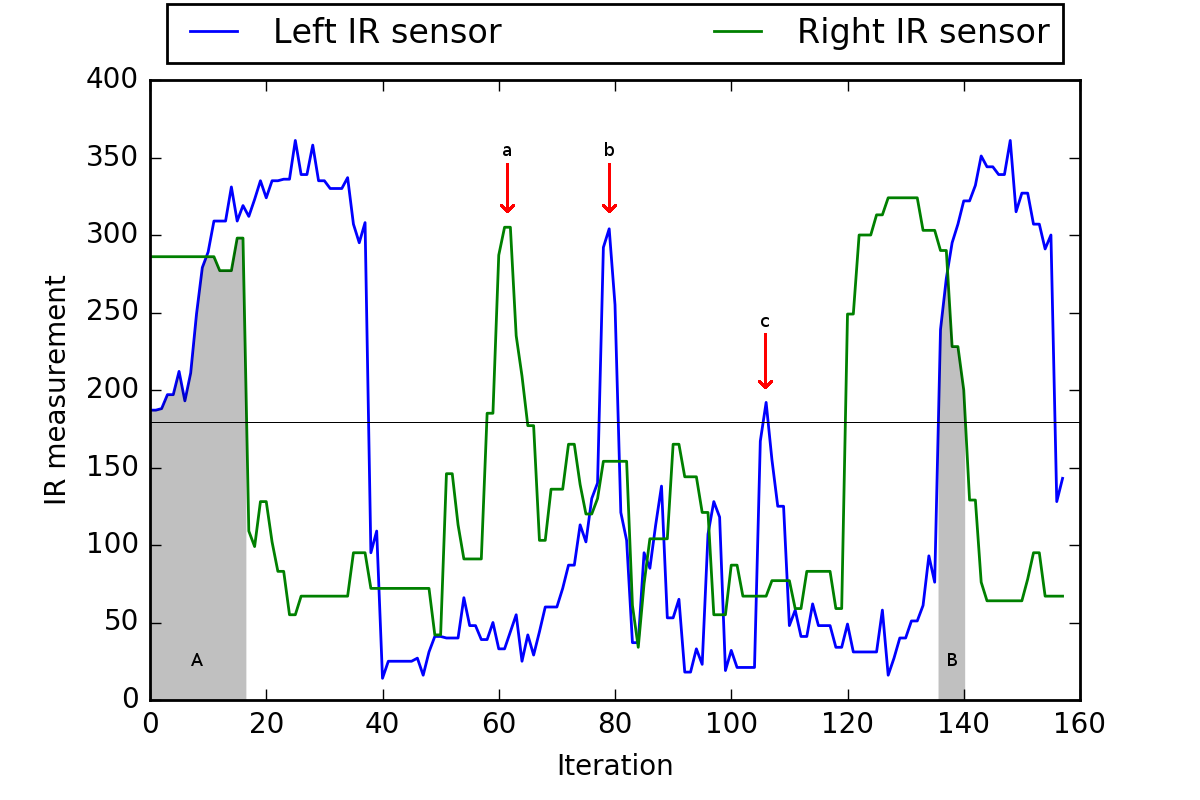
\includegraphics[width=0.7\linewidth]{res/360-scan-plot.png}
    \caption{}
    \label{fig:}
\end{figure}

\newpage
